\documentclass{article}

\usepackage{graphicx}
\usepackage{tikz}
\usepackage{tikzsymbols}
\usetikzlibrary{calc,patterns,shapes.geometric}
\pagestyle{empty}
\usepackage[margin=0pt]{geometry}
\geometry{papersize={14in,12in}}

\def\centerarc[#1](#2)(#3:#4:#5){\draw[#1] ($(#2)+({#5*cos(#3)},{#5*sin(#3)})$) arc (#3:#4:#5);}

\begin{document}
	\begin{figure}
		\centering
		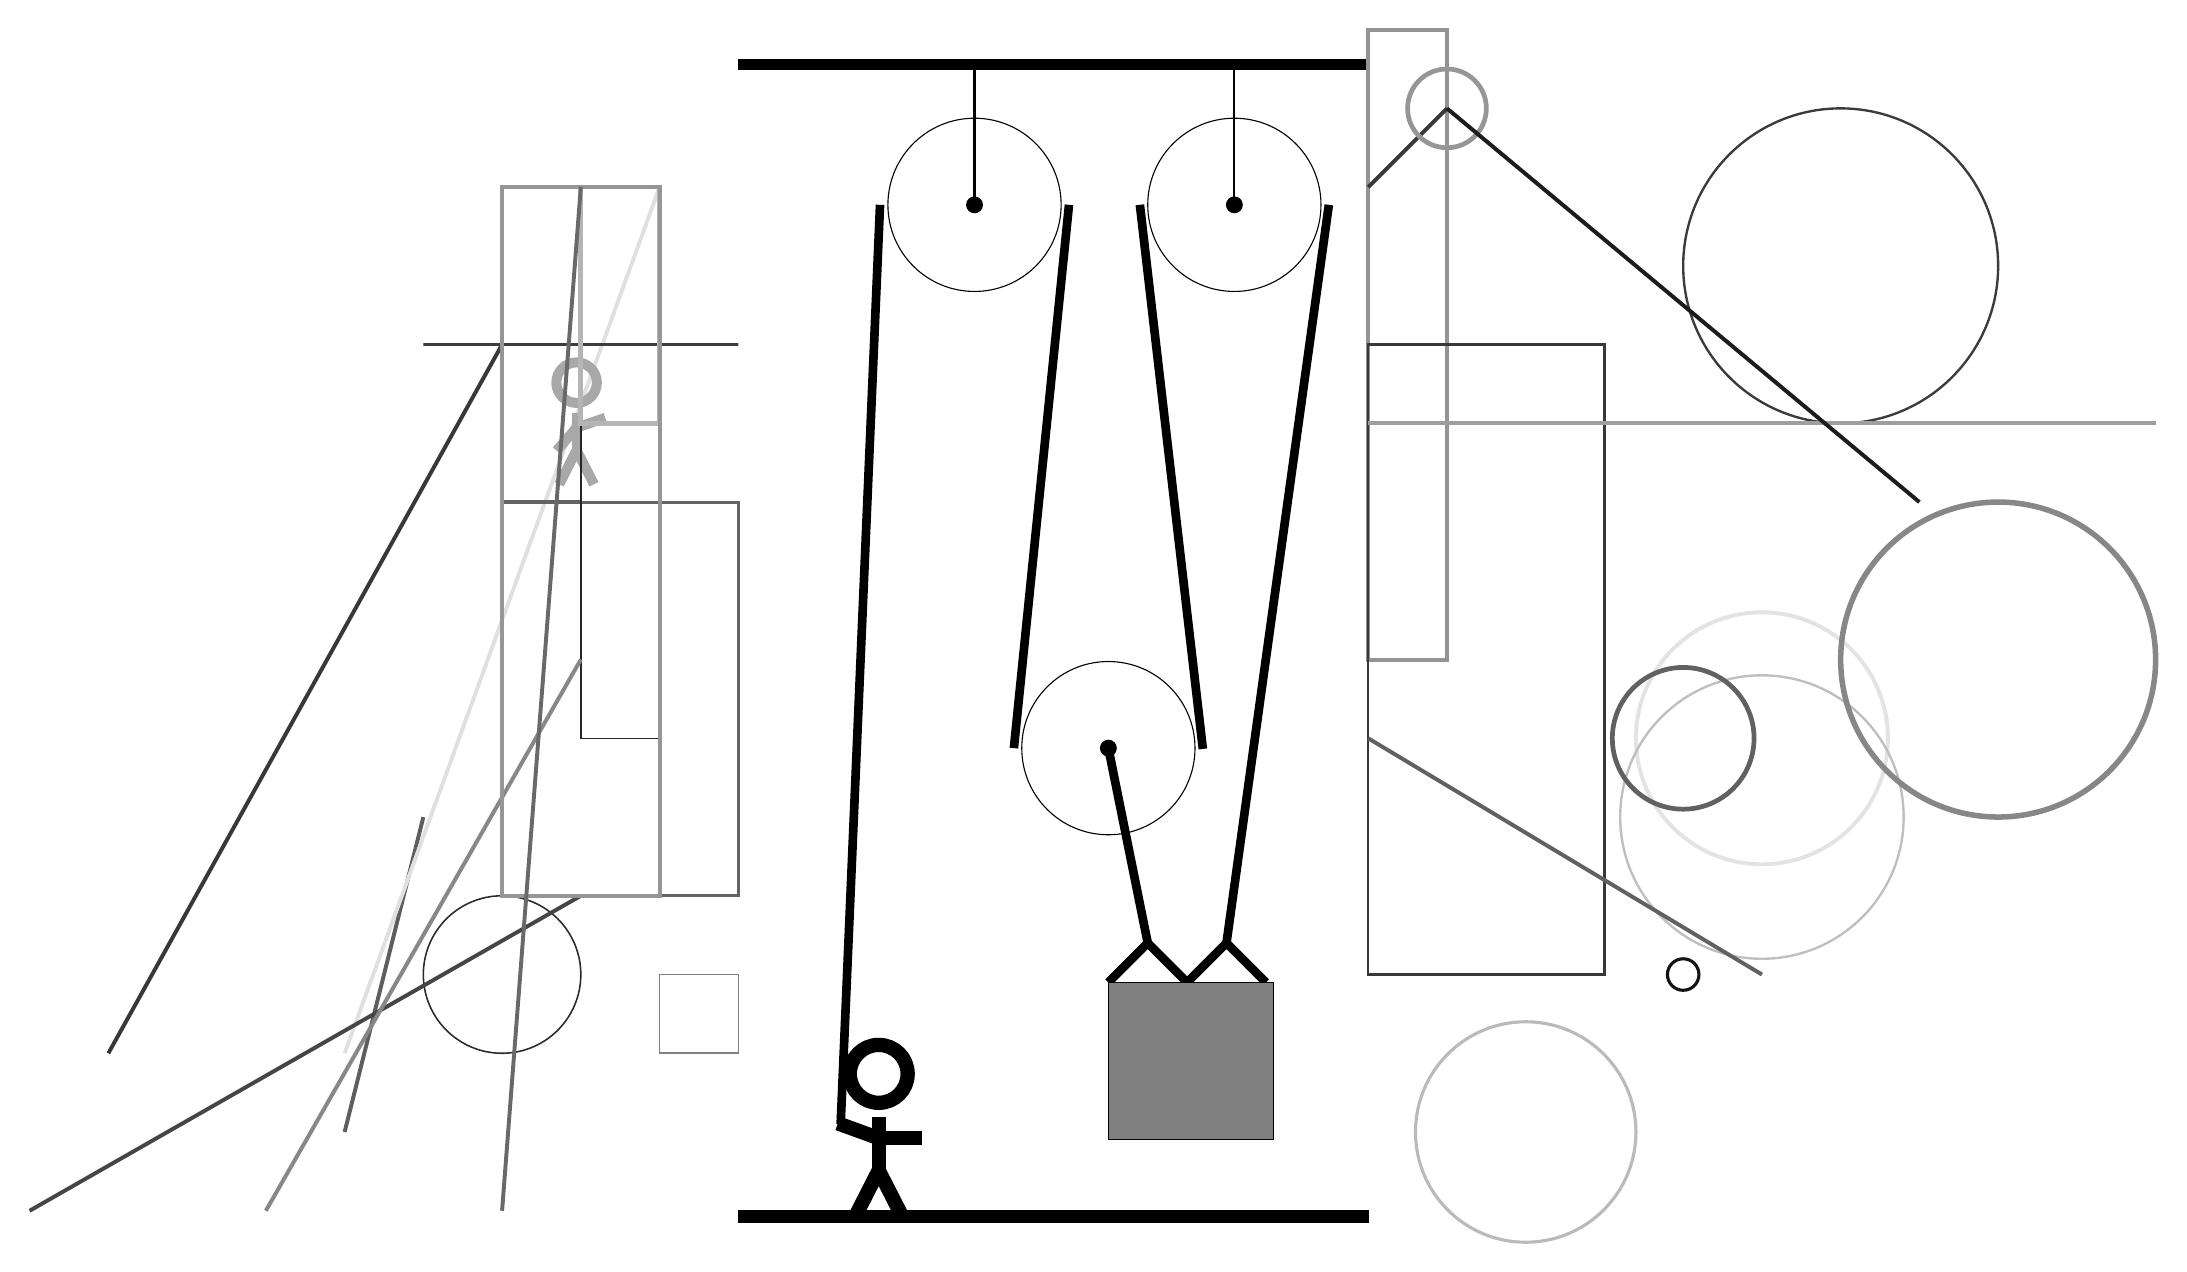
\begin{tikzpicture}
			%%%%% START %%%%%
			
			\draw[fill=black] (-2, 11.5) rectangle (6, 11.625);
			
			\draw (1, 9.775) circle (1.1);
			\draw[fill=black] (1, 9.775) circle (0.1);
			\draw[thick] (1, 9.775) -- (1, 11.5);
			
			\draw[line width=0.2mm, color=black!50] (-3, 0) rectangle (-2, -1);
			
			\draw[line width=0.5mm, color=black!63](-7, -2) -- (-6, 2);
			\draw[line width=0.5mm, color=black!12](-7, -1) -- (-3, 10);
			\draw[line width=0.5mm, color=black!42] (6, 4) rectangle (7, 12);
			
			\draw [line width=0.5mm, color=black!11](11, 3) circle (1.6);
			\draw [line width=0.3mm, color=black!77](12, 9) circle (2.0);
			\node[line width=0.2mm, color=black!34] at (-4, 7) {\Strichmaxerl[7][49][19]};
			\draw [line width=0.3mm, color=black!25](11, 2) circle (1.8);
			\draw[line width=0.5mm, color=black!62](-4, 6) -- (-5, 6);
			\draw[line width=0.4mm, color=black!76] (-2, 8) rectangle (-6, 8);
			\draw [line width=0.7mm, color=black!47](14, 4) circle (2.0);
			
			\draw [line width=0.2mm, color=black!83](-5, 0) circle (1.0);
			\draw[line width=0.3mm, color=black!78] (6, 8) rectangle (9, 0);
			
			\draw[line width=0.5mm, color=black!78](6, 10) -- (7, 11);
			\draw[line width=0.4mm, color=black!61] (-2, 6) rectangle (-5, 1);
			\draw [line width=0.4mm, color=black!92](10, 0) circle (0.2);
			\draw[line width=0.5mm, color=black!62](11, 0) -- (6, 3);
			\draw[line width=0.2mm, color=black!85] (-4, 3) rectangle (-3, 10);
			\draw[line width=0.5mm, color=black!73](-4, 1) -- (-11, -3);
			\draw [line width=0.6mm, color=black!62](10, 3) circle (0.9);
			\draw[line width=0.5mm, color=black!78](-5, 8) -- (-10, -1);
			
			\draw[line width=0.5mm, color=black!38](6, 7) -- (16, 7);
			\draw [line width=0.6mm, color=black!41](7, 11) circle (0.5);
			\draw [line width=0.4mm, color=black!27](8, -2) circle (1.4);
			\draw[line width=0.5mm, color=black!89](7, 11) -- (13, 6);
			
			\draw[line width=0.6mm, color=black!29] (-4, 10) rectangle (-3, 7);
			\draw[line width=0.5mm, color=black!47](-4, 4) -- (-8, -3);
			\draw[line width=0.5mm, color=black!41] (-3, 10) rectangle (-5, 1);
			\draw[line width=0.5mm, color=black!59](-4, 10) -- (-5, -3);
			
			\draw (4.3, 9.775) circle (1.1);
			\draw[fill=black] (4.3, 9.775) circle (0.1);
			\draw[thick] (4.3, 9.775) -- (4.3, 11.5);
			
			\draw (2.7, 2.875) circle (1.1);
			\draw[fill=black] (2.7, 2.875) circle (0.1);
			
			\draw[line width=1.1mm]  (2.7, -0.1) -- (3.2, 0.4) -- (3.7, -0.1) -- (4.2, 0.4) -- (4.7, -0.1);
			\draw[fill=black!50] (2.7, -0.1) rectangle (4.8, -2.1);
			
			\draw[line width=1.1mm](-0.7, -1.9) -- (-0.2, 9.775);
			\centerarc[line width=1.1mm](1, 9.775)(0:180:1.2000000000000002);
			\draw[line width=1.1mm](2.2, 9.775) -- (1.5, 2.875);
			\centerarc[line width=1.1mm](2.7, 2.875)(180:370:1.2000000000000002);
			\draw[line width=1.1mm] (3.9, 2.865) -- (3.1, 9.775);
			\centerarc[line width=1.1mm](4.3, 9.775)(0:180:1.2000000000000002);
			\draw[line width=1.1mm](4.2, 0.4) -- (5.5, 9.775);
			\draw[line width=1.1mm] (3.2, 0.4) -- (2.7, 2.875);
			
			\node at (-0.2, -2) {\Strichmaxerl[10][-20][0]};
			
			\draw[fill=black] (-2, -3) rectangle (6, -3.15);
			
			%%%%% END %%%%%
		\end{tikzpicture}
	\end{figure}	
\end{document}